\documentclass[11pt]{article}
\usepackage[margin=0.8in]{geometry}
\usepackage{amsmath,amssymb,graphicx,xurl,hyperref}
\hypersetup{colorlinks=true,urlcolor=blue}
\setlength{\parindent}{0pt}\setlength{\parskip}{6pt}
\begin{document}
{\LARGE Actual source taper and exact jet determination}\par
November 9, 2026. Mathematical source \texttt{31c212f5a}.\par
Unsigned producer evidence throughout [pcc:unverified].

\textbf{Result.}
The actual nonzero source grid nodes are now counted by exact two-adic
valuation. Their source ceiling taper has enough total multiplicity for
the repaired polynomial's doubled degree. Exact scaled source jets determine
the actual cleared packed polynomial over every $\mathbb Q$-algebra, including
nilpotent coefficient rings. This continues the preceding affine-contraction
component and does not replace its versioned report.

\textbf{Actual grid counts.}
Let $L=2^a$ and $m\in\operatorname{Fin}(2^{a+1})$, with actual source point
$t_m=m-2^a\in\mathbb Z$. For each active $i<a$, an explicit quotient/remainder
bijection counts the residue class $m\bmod 2^{i+1}=2^i$. Since $2^{i+1}\mid L$,
shifting by $L$ preserves it. The integer lemma
\[
 t\bmod 2^{i+1}=2^i\quad\Longleftrightarrow\quad
 t\ne0\ \text{and}\ v_2(t)=i
\]
therefore gives exactly $2^{a-i}$ actual nodes. Zero is excluded explicitly;
the convention for valuation at zero is not used as a source level.

\textbf{Actual ceiling and all-level multiplicity.}
The source ceiling $h=\lceil3M/u\rceil$ has its budget $3M\leq hu$ derived.
Define $q(0)=0$ and $q(t)=h\max(0,u-v_2(t))$ otherwise. The Lean proof identifies
its sum over individual actual grid nodes with the complete level sum
\[
 \sum_m q(t_m)=\sum_{i=0}^{u-1}2^{a-i}h(u-i).
\]
For $3\leq u\leq a$ and $u\leq M$, this satisfies
\[
 \sum_m q(t_m)>2M(2L-1).
\]
The first three actual levels certify a lower bound on this full sum.
The source's ceiling and actual cardinalities are derived; no assumed
level distribution or user-supplied budget replaces them. The odd-node lower
bound alone would not justify the doubled degree.

\textbf{Exact uniqueness.}
For nodes with unit pairwise differences over a commutative ring, the factors
$(X-t_i)$ are pairwise coprime. Equality of exact Taylor coefficients below
$q_i$ implies $(X-t_i)^{q_i}\mid F-G$. Their monic product divides $F-G$ and
has degree $\sum_iq_i$. If both polynomial degrees are below that sum, then
$F-G=0$. This proof permits zero divisors and nilpotents.

Distinct actual source nodes have nonzero rational differences, which map to
units in any $\mathbb Q$-algebra. The actual chart is $t+2Lz$; its coefficient
of order $j$ equals Taylor coefficient $j$ times $(2L)^j$. This unit scaling
connects actual scaled jets to the actual cleared packed polynomial's degree
bound and gives the advertised determination theorem.
\newpage
\textbf{Precision boundary.}
Scaling cancellation uses the $\mathbb Q$-algebra, where $2L$ is a unit.
It cannot be repeated modulo $2^p$. This component proves exact determination;
finite-precision reconstruction, construction costs, efficient evaluation of
the contraction and a recursive bit-cost bound remain separate obligations.

\begin{center}
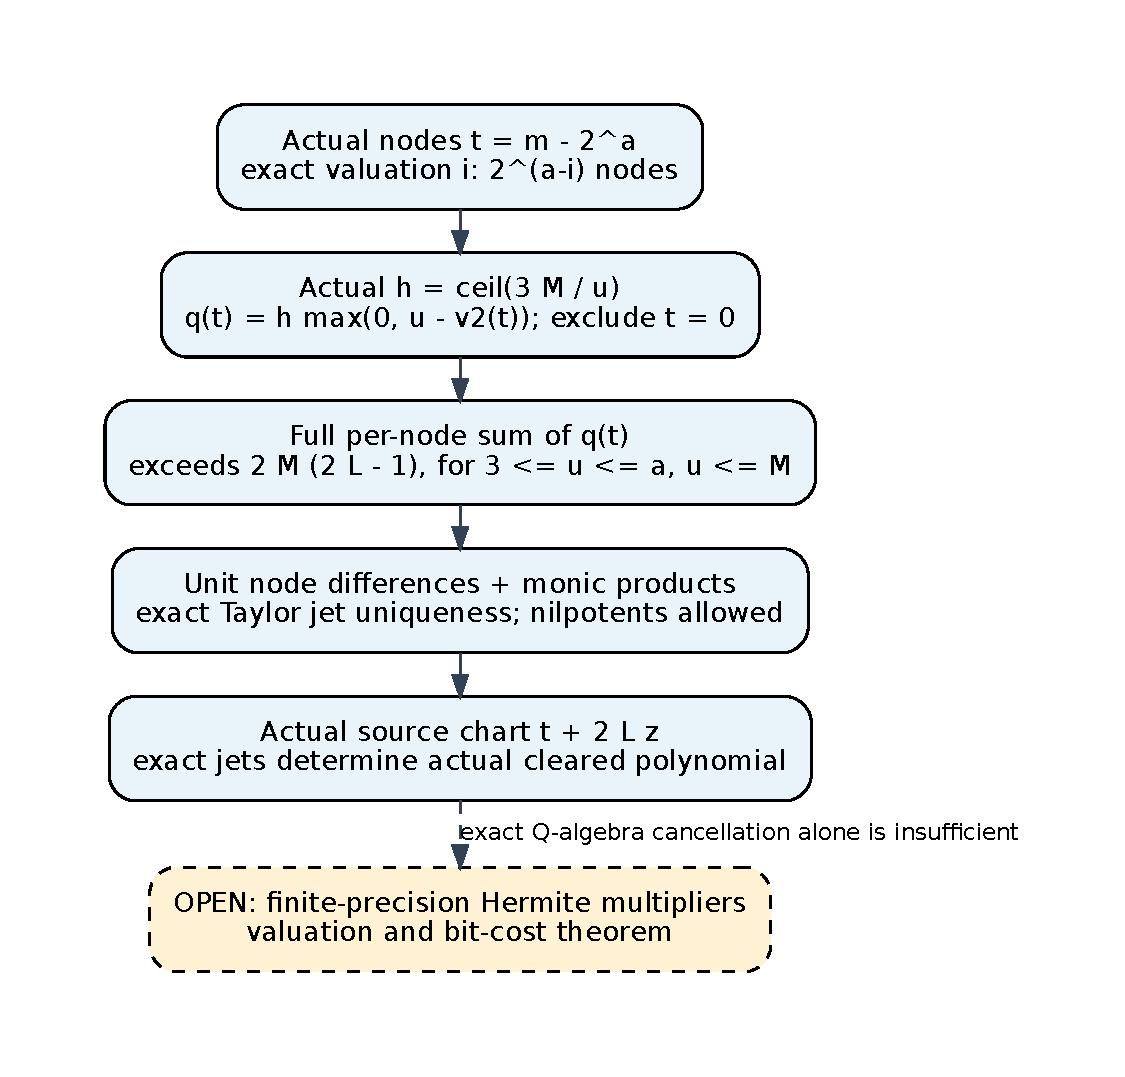
\includegraphics[width=0.98\textwidth,height=0.54\textheight,keepaspectratio]{bridge.pdf}
\end{center}
Solid boxes describe this component; the dashed box remains open.

\textbf{Checks.}
Both modules are default targets. The default build passed, and the actual
source-discovering gate reports 162 declarations with zero extra trusted axioms.

Foundations remain \texttt{propext}, \texttt{Classical.choice}, \texttt{Quot.sound}.
The import-inclusive fresh replay checks \texttt{HermiteUniqueness}.
Its status is in \path{lean/recovery-fresh-status.json}, with the raw log beside it.
All checks remain unsigned producer evidence [pcc:unverified].

Pinned toolchain: Lean 4.35.0. CryptoLean:
\path{148f5dc389b341401e06d76abe7783c4ccf42f2e}. Mathlib:
\path{cfc55fc58714a59dc06e6e79edc6d1d95140d3c2}.
No checker, proof gate, kernel, trust policy or dependency revision changed.
Failed node/API elaborations and both passing Hermite builds are retained.
No timing or performance inference is drawn from compiler logs. Earlier plots
and scoreboards remain historical because no measured value changed.
\newpage
\textbf{Proof map and unsigned records.}
Canonical statement hashes are in \path{lean/recovery-claim-pins.json}.

\begin{tabular}{p{0.30\textwidth}p{0.62\textwidth}}
Actual nonzero level count & \texttt{NodeMultiplicity.actualValuationCard}\newline PCC-20261109-ed63ef\\[6pt]
Actual ceiling/per-node margin & \texttt{NodeMultiplicity.sourceJetDegreeMargin}\newline PCC-20261109-966d63\\[6pt]
Exact ring-valued uniqueness & \texttt{HermiteUniqueness.exactHermiteUnique}\newline PCC-20261109-7e8217\\[6pt]
Actual packed scaled jets & \texttt{HermiteUniqueness.}\newline\texttt{actualPackedScaledJetsDetermine}\newline PCC-20261109-05e9da
\end{tabular}

The identities involve finite counted sets, valuations and variable-length jet
vectors. They do not fit polynomial-expression certificate schema v1; their
evidence is the quantified Lean source and source audit. The preceding affine
polynomial certificate is unchanged.

\textbf{Sources and scope.}
Reviewed OpenAI, \emph{The Exponential Time Hypothesis is False}, October 25,
2026, D.4.3--D.4.4 and D.8--D.10, plus the repository's
\texttt{matched-recovery-independent.md} and actual Mathlib remainder, ceiling,
Taylor, coprime-product and monic-degree APIs. Primary PDF SHA256:
\path{5b1612dc2eebb2cad5b4cbe62d1fed2982f01ab1908c26f70010a651487e8123}.
Pinned source:
\url{https://github.com/openai/math/blob/7ef5c0cc5ca4b0e072b7a050fca09ab24bc6fa3a/preprints/The-Exponential-Time-Hypothesis-is-False-October-25-2026/paper.pdf}.
The KB MCP is absent and repository fallback unavailable (exit 127). This is
a bounded source review and formalization of established interpolation, with
no novelty or exhaustion claim. No curve or subgroup solve was attempted.

\textbf{Next discriminating proof.}
Formalize the actual normalized Hermite basis $E_t$ from D.9 and bound its
multiplier valuations. D.10 uses the weighted level difference with factor
$j/2^j$; omitting $j$ gives the wrong series. Its taper inequality yields
$v_2(E_t(0))\geq-6hD_i$ via $\sum_{j\geq1}j^2/2^j=6$.
Derive the actual ceiling upper bound $hu\leq4M$, bound evaluation at
$-t/(2L)$ and propagate errors using $p_i=p+8hD_i+8M(a+1)$.
Those bounds do not follow from exact uniqueness alone.

A later test should distinguish this actual precision from the old doubled-budget
proxy. It requires a separately prospective protocol and the precision proof
before changing any campaign conclusion. The completed frozen panel was not
rerun or relabelled, and no loss was attributed to host load.

\textbf{Reproduction.}
With the pinned toolchain on PATH, from the repository root:
\begin{quote}\small\ttfamily
lake -d research/prime\_common\_scalar\_20261108/lean build\par
lake -d research/prime\_common\_scalar\_20261108/lean \textbackslash\par
\quad env leanchecker --fresh --verbose HermiteUniqueness
\end{quote}
The source gate receipts, exact commands, failed attempts and statement pins
are included alongside the sources. No performance or benchmark row is promoted.
\end{document}
